%!TEX root = ../../../../thesis.tex
\section{Natural Computing}

	For a long time the terms \emph{Nature} and \emph{Computing} used to denote terms which could hardly be any more opposite to each other. Starting with the mid 1940s this perception began to fade gradually when researchers started to explore the exciting possibility of merging ideas from computing and nature. The search for new problem solving techniques, novel approaches to synthesize natural phenomena in silico as well as novel natural materials to perform computation began. Today, the pursuit of these three distinct yet interrelated approaches is known as \emph{Natural Computing}~\cite{de2005natural,de2006fundamentals}.

	In this section we give a short introduction to the scope of Natural Computing and mention its most important areas of interest. Our exposition closely follows de~Castro~\cite{de2007fundamentals} who describes natural computing as the extraction of ideas from nature to develop computational systems, or using natural materials to perform computation. He suggest to divide the field into three main areas:

	\begin{description}
		\item[a)] Computing inspired by nature
		\item[b)] The simulation and emulation of nature by means of computing
		\item[c)] Computing with natural materials
	\end{description}

	\begin{figure}
			\centering
			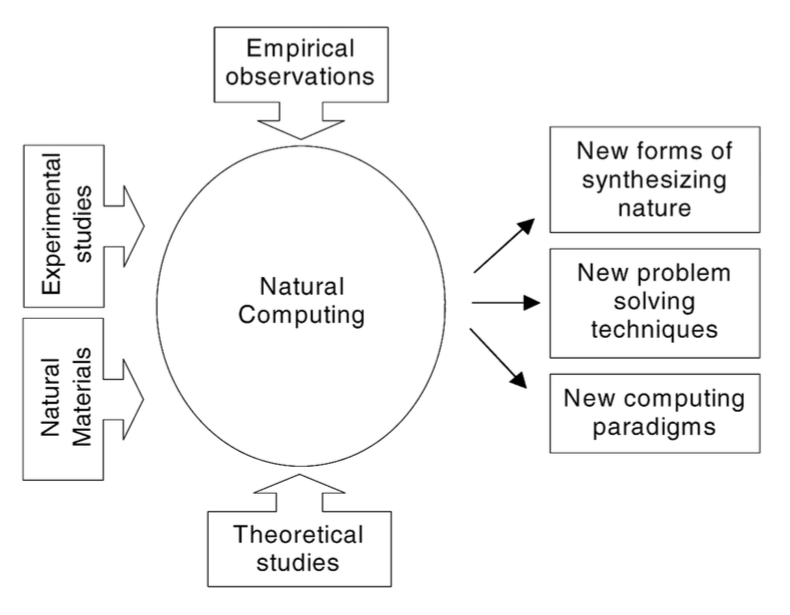
\includegraphics[width=\linewidth,keepaspectratio]{natural_computing.png}
			\caption[The goals of natural computing.]{A schematic of the components and goals of natural computing.}
			\label{fig:natural_computing}
	\end{figure}

	\Fref{fig:natural_computing} illustrates the goals of natural computing. The study of these three highly entangled areas seamlessly merge empirical observations and theoretical studies from diverse fields such as biology, physics, chemistry, engineering and computer science amongst others. Thus it is vital for researchers to be open, collaborate and share their ideas and knowledge in order to meet the challenges posed by the highly interdisciplinary field that is natural computing.